\PassOptionsToPackage{obeyspaces,spaces}{url}
\documentclass[10pt,a4paper]{article}
% ---------------------------------------------------------------------------
%  Project Dossier -- Lightweight Programmable Packet Processing on STM32
%  Compiles with pdflatex (Overleaf: default settings).
% ---------------------------------------------------------------------------
\usepackage[T1]{fontenc}
\usepackage[utf8]{inputenc}
\usepackage{charter}
\usepackage[scaled=0.90]{helvet}
\renewcommand{\ttdefault}{txtt}
\usepackage[expansion=false]{microtype}
\usepackage[a4paper,margin=2.1cm,headheight=19pt]{geometry}
\usepackage{xcolor}
\usepackage{booktabs,tabularx,array,longtable,colortbl}
\usepackage{enumitem}
\usepackage{titlesec}
\usepackage{fancyhdr}
\usepackage{amsmath}
\usepackage{tikz}
\usetikzlibrary{arrows.meta,positioning,calc,fit,backgrounds,decorations.pathreplacing}
\usepackage[most]{tcolorbox}
\usepackage{listings}
\usepackage{caption}
\usepackage[hidelinks]{hyperref}

% ---------------- colours ----------------
\definecolor{ink}{HTML}{1B2430}
\definecolor{accent}{HTML}{0F5C6E}
\definecolor{accentlight}{HTML}{E3F0F2}
\definecolor{muted}{HTML}{5A6472}
\definecolor{warn}{HTML}{A23B1E}
\definecolor{warnlight}{HTML}{FBEDE8}
\definecolor{ok}{HTML}{2D6A3E}
\definecolor{oklight}{HTML}{E8F3EA}
\definecolor{rule}{HTML}{C9D1D9}
\definecolor{hwfill}{HTML}{EEF1F4}
\definecolor{isrfill}{HTML}{FDF1D8}
\definecolor{taskfill}{HTML}{E6EEF7}
\definecolor{hookfill}{HTML}{DDF0EC}
\definecolor{dropfill}{HTML}{F8E1DA}
\color{ink}

% ---------------- headings ----------------
\titleformat{\section}{\sffamily\Large\bfseries\color{accent}}{\thesection}{0.6em}{}
\titleformat{\subsection}{\sffamily\large\bfseries\color{ink}}{\thesubsection}{0.5em}{}
\titleformat{\subsubsection}{\sffamily\normalsize\bfseries\color{ink}}{}{0em}{}
\titlespacing*{\section}{0pt}{16pt}{6pt}
\titlespacing*{\subsection}{0pt}{11pt}{4pt}
\titlespacing*{\subsubsection}{0pt}{8pt}{2pt}

\pagestyle{fancy}
\fancyhf{}
\fancyhead[L]{\sffamily\footnotesize\color{muted} MTP Project Dossier --- Programmable Packet Processing on STM32}
\fancyhead[R]{\sffamily\footnotesize\color{muted} Status: 28 Oct 2026}
\fancyfoot[C]{\sffamily\footnotesize\color{muted}\thepage}
\renewcommand{\headrulewidth}{0.4pt}
\renewcommand{\headrule}{\hbox to\headwidth{\color{rule}\leaders\hrule height \headrulewidth\hfill}}

\setlist{itemsep=2pt,topsep=3pt,parsep=0pt,leftmargin=1.3em}
\setlength{\parindent}{0pt}
\setlength{\parskip}{5pt}
\renewcommand{\arraystretch}{1.22}
\captionsetup{font={small,sf},labelfont={bf,color=accent}}

\usepackage{url}
\usepackage{needspace}
\DeclareUrlCommand\code{\urlstyle{tt}}
\makeatletter\g@addto@macro\UrlBreaks{\do\_\do\(\do\,\do\>}\makeatother
\newcommand{\done}{\textcolor{ok}{\textbf{done}}}
\newcommand{\open}{\textcolor{warn}{\textbf{open}}}
\newcolumntype{L}{>{\raggedright\arraybackslash}X}
\newcolumntype{P}[1]{>{\raggedright\arraybackslash}p{#1}}

\newtcolorbox{keybox}[1]{enhanced,colback=accentlight,colframe=accent,boxrule=0.6pt,arc=2pt,
  left=6pt,right=6pt,top=4pt,bottom=4pt,fonttitle=\sffamily\bfseries\small,
  title=#1,coltitle=white,colbacktitle=accent,breakable}
\newtcolorbox{warnbox}[1]{enhanced,colback=warnlight,colframe=warn,boxrule=0.6pt,arc=2pt,
  left=6pt,right=6pt,top=4pt,bottom=4pt,fonttitle=\sffamily\bfseries\small,
  title=#1,coltitle=white,colbacktitle=warn,breakable}
\newtcolorbox{okbox}[1]{enhanced,colback=oklight,colframe=ok,boxrule=0.6pt,arc=2pt,
  left=6pt,right=6pt,top=4pt,bottom=4pt,fonttitle=\sffamily\bfseries\small,
  title=#1,coltitle=white,colbacktitle=ok,breakable}

\lstdefinestyle{bc}{basicstyle=\ttfamily\footnotesize,columns=fullflexible,keepspaces=true,
  backgroundcolor=\color{hwfill},frame=single,rulecolor=\color{rule},framesep=4pt,
  xleftmargin=4pt,xrightmargin=4pt,commentstyle=\color{muted}\itshape,
  morecomment=[l]{;},showstringspaces=false,aboveskip=6pt,belowskip=4pt}

\begin{document}

% =====================================================================
% Title block
% =====================================================================
\thispagestyle{empty}
\vspace*{1.2cm}
{\sffamily\color{accent}\small\bfseries MTECH PROJECT (MTP) --- PROJECT DOSSIER\par}
\vspace{6pt}
{\raggedright\sffamily\bfseries\fontsize{21}{26}\selectfont Lightweight Programmable Packet Processing Framework \& Execution Layer for STM32-Based RTOS\par}
\vspace{10pt}
{\large An XDP/eBPF-inspired, verified bytecode VM in the Ethernet receive path of FreeRTOS + lwIP on a Cortex-M33\par}
\vspace{16pt}
\begin{tabularx}{\textwidth}{@{}P{3.3cm}L@{}}
\toprule
\textsf{\textbf{Team}} & Kiran (2025EET2800) --- Role 1: VM \& Dynamic Execution Layer \\
 & Nishant (2025EET2734) --- Role 2: XDP-Inspired Packet Processing \& RTOS Integration \\
\textsf{\textbf{Supervisor}} & Prof.\ Kaushik Saha \\
\textsf{\textbf{Board}} & NUCLEO-H563ZI (STM32H563ZIT6, Arm Cortex-M33 @ 250\,MHz) \\
\textsf{\textbf{Software}} & FreeRTOS, lwIP, STM32H5 HAL \\
\textsf{\textbf{Status as of}} & 28 October 2026 (after the 24 Sep 2026 mid-term evaluation) \\
\bottomrule
\end{tabularx}

\vspace{14pt}
\begin{keybox}{How to use this dossier}
This is the single reference for everything known about the project so far: what you are building and why, the board, the architecture, who does what, what has been done and verified, what is broken, the literature, the evaluation plan, the roadmap to the final thesis, resume material, and viva preparation. It ships with a repository bundle (\code{MTP_XDP_STM32/}) and a \code{CLAUDE.md} so the work continues cleanly in Claude Code (Section~\ref{sec:claudecode}).

Facts marked \emph{verified} were checked on 28 Oct 2026 against vendor sources (STM32H5 HAL v1.7.0, lwIP 2.2.x, FreeRTOS-Kernel headers), by compiling, or by running tests. Nothing in this document has been run on your physical board by me. Hardware results must come from you.
\end{keybox}

\vspace{6pt}
{\sffamily\small\bfseries\color{accent} Contents}\par
\begin{small}
\begin{tabularx}{\textwidth}{@{}L L@{}}
1\enspace Project at a glance & 9\enspace Literature: studied, recommended, positioning \\
2\enspace Problem, idea, research questions & 10\enspace Evaluation plan \\
3\enspace Hardware \& software platform & 11\enspace Roadmap to the final thesis \\
4\enspace System architecture & 12\enspace Resume \& interview material \\
5\enspace Division of work & 13\enspace Viva / evaluation Q\&A preparation \\
6\enspace What you shared, and project history & 14\enspace Continuing in Claude Code \\
7\enspace What has been built and verified & A\enspace Bundle inventory \quad B\enspace ISA opcode table \\
8\enspace Known issues and deck-vs-code gaps & References \\
\end{tabularx}
\end{small}

\newpage
% =====================================================================
\section{Project at a glance}
% =====================================================================
\begin{tabularx}{\textwidth}{@{}P{3.6cm}L@{}}
\toprule
\textbf{One-line pitch} & Bring the Linux \textbf{XDP + eBPF} idea (programmable, verified, earliest-possible packet filtering in the driver) to a \textbf{microcontroller running FreeRTOS + lwIP}, and measure where in the RTOS receive path such filtering pays off. \\
\textbf{Core mechanism} & A heap-free bytecode VM (64-bit instructions, 8 registers) runs a verified filter program on each received Ethernet frame \emph{in place} (zero-copy) and returns PASS or DROP. \\
\textbf{Hook 1 (proposed)} & Driver layer: inside the STM32H5 HAL receive path (\code{HAL_ETH_RxLinkCallback}), \emph{before} lwIP ever sees the frame. A dropped frame's buffer goes straight back to the RX pool. \\
\textbf{Hook 2 (baseline)} & lwIP layer: \code{LWIP_HOOK_IP4_INPUT} inside \code{ip4_input()}, after the frame has crossed into lwIP's \code{tcpip_thread}. \\
\textbf{Baselines} & No filter; the same filter in native C at both hooks; the MAC's hardware L3/L4 filter. \\
\textbf{Demo} & DDoS prototype: drop a UDP flood aimed at a target port while legitimate traffic keeps flowing. \\
\textbf{Metrics} & Packet latency, throughput / drop rate, CPU utilisation, RAM/flash footprint, RTOS timing overhead. \\
\textbf{Where you are} & Mid-term passed (24 Sep 2026). VM engine compiles and passes 33 host tests. The driver-layer hook needs fixes before it can run (Section~\ref{sec:issues}). No hardware results yet. \\
\bottomrule
\end{tabularx}

% =====================================================================
\section{Problem, idea and research questions}
% =====================================================================
\subsection{The problem}
\begin{itemize}
  \item \textbf{RTOS network stacks spend resources before deciding.} In lwIP every received frame is wrapped in a \code{pbuf}, handed to \code{tcpip_thread} through a mailbox (a context switch), demultiplexed by \code{ethernet_input()}, and only then parsed by \code{ip4_input()}. Under a flood, the MCU burns its cycle budget on packets it will throw away, which is the classic \emph{receive livelock} problem \cite{mogul97}.
  \item \textbf{Filtering logic is frozen at compile time.} Changing a firewall rule on an MCU normally means rebuilding and reflashing firmware.
  \item \textbf{Running updatable logic in the kernel is dangerous.} An MCU has no process isolation. A buggy or malicious filter that loops or dereferences a bad pointer takes the whole node down.
  \item \textbf{Heavier sandboxes do not fit.} Linux XDP needs a Linux kernel. WebAssembly runtimes on MCUs cost tens of KiB of RAM (e.g.\ $\sim$85\,KiB for WASM3 in the measurements of \cite{fc21}).
\end{itemize}

\subsection{The idea}
Port the XDP pattern \cite{xdp18} to an MCU: hook the \emph{earliest} software point in the Ethernet receive path, run a small \emph{verified} bytecode program there, and drop unwanted frames before the stack pays for them. The VM borrows from BPF \cite{bpf93} and the MCU-focused rBPF / Femto-Containers line of work \cite{rbpf20,fc21,fc22}: a register-based ISA, a static verifier that guarantees termination, runtime bounds checks on packet access, and no heap.

\subsection{Research questions}
\begin{description}[leftmargin=2.6em,style=nextline,itemsep=3pt]
  \item[RQ1] \textbf{Placement.} How much CPU time and latency does dropping at the driver layer save compared with dropping at lwIP's \code{ip4_input()}?
  \item[RQ2] \textbf{Interpretation cost.} What does a verified VM cost compared with native C for the same filter on a Cortex-M33? Is the cost per-packet (entry, checks) or per-instruction (dispatch)?
  \item[RQ3] \textbf{Verification for speed.} Can the verifier statically prove a minimum frame length, so runtime bounds checks disappear? How much does that save?
  \item[RQ4] \textbf{Survivability.} Under a UDP flood of rising rate, how much legitimate traffic (goodput, RTT) survives in each configuration, and where does receive livelock set in?
\end{description}

\subsection{Intended contributions (what the thesis will claim, \emph{once measured})}
\begin{enumerate}[label=\textbf{C\arabic*},leftmargin=2.2em]
  \item An XDP-style programmable ingress hook in the STM32H5 HAL Ethernet receive path of FreeRTOS + lwIP, with zero-copy verdicts and immediate buffer recycling on drop.
  \item A compact verified VM for packet filtering on Cortex-M33: custom 64-bit ISA, a forward-only-CFG verifier (termination), and memory safety by construction plus runtime checks, all heap-free in about 1\,KB of flash.
  \item A controlled comparison that separates the \emph{placement effect} (driver vs lwIP hook) from the \emph{interpretation overhead} (VM vs native C), with hardware filtering as a lower bound.
  \item (Planned) Verifier-driven elimination of runtime bounds checks, and safe runtime replacement of filter programs without reflashing.
\end{enumerate}

\begin{keybox}{Honest novelty statement (use this framing with examiners)}
Early drop and verified bytecode are known ideas (XDP, BPF, rBPF, Femto-Containers). The contribution is putting them \emph{together} on a commodity MCU's high-speed Ethernet DMA path under FreeRTOS + lwIP, and \emph{quantifying} placement vs interpretation vs fixed-function hardware. Prior MCU VM work targeted low-rate wireless IoT and generic OS hooks. The strength of the thesis will come from the quality of the measurements.
\end{keybox}

% =====================================================================
\section{Hardware and software platform}
% =====================================================================
\subsection{Board and MCU (verified)}
\begin{tabularx}{\textwidth}{@{}P{4.1cm}L@{}}
\toprule
Board & \textbf{NUCLEO-H563ZI} (Nucleo-144). On-board debugger \textbf{ST-LINK/V3EC} (SWD, virtual COM port) \\
MCU & \textbf{STM32H563ZIT6} (LQFP144) \\
Core & Arm \textbf{Cortex-M33} (Armv8-M Mainline) with TrustZone and FPU, up to \textbf{250\,MHz} \\
Memory & \textbf{2\,MB} flash, \textbf{640\,KB} SRAM \\
Ethernet & 10/100 Ethernet MAC with dedicated DMA, \textbf{RMII} to an on-board \textbf{LAN8742} PHY, RJ45 \\
User I/O & LEDs LD1 = PB0 (green), LD2 = PF4 (yellow), LD3 = PG4 (red); USER button = PC13 \\
Key documents & RM0481 (reference manual), UM3115 (Nucleo user manual), STM32H5 HAL ETH driver \\
\bottomrule
\end{tabularx}

\subsection{Hardware features that matter for the research (verified in HAL/CMSIS headers)}
\begin{itemize}
  \item \textbf{DWT cycle counter} (\code{DWT->CYCCNT}): cycle-accurate timing of the filter (RQ1--RQ3).
  \item \textbf{MAC hardware L3/L4 filter}: 2 filter slots matching IPv4/IPv6 addresses and TCP/UDP ports (\code{HAL_ETHEx_SetL3FilterConfig}, \code{HAL_ETHEx_SetL4FilterConfig}). It can do the \emph{basic} DDoS demo with zero CPU, so an examiner will ask about it. Use it as baseline C5 and make the VM do what it cannot (rate limiting, port lists, header logic).
  \item \textbf{RX missed-frame counter} (\code{ETH->DMACMFCR}): counts frames lost because no RX buffer was free, a direct livelock indicator (RQ4).
  \item \textbf{TrustZone}: optional future isolation of the VM (stretch goal).
\end{itemize}

\subsection{Software stack, and one important caveat}
\begin{warnbox}{STM32CubeMX does not generate lwIP for STM32H5}
For the H5 family, CubeMX/CubeIDE offers no lwIP middleware (confirmed in ST community threads as recently as March 2026). ST's route is the GitHub package \code{stm32h5-classic-coremw-apps} (clone with \code{--recursive}), which contains lwIP examples for NUCLEO-H563ZI and an \code{ethernetif.c} with a zero-copy RX pool. ST's guide used STM32CubeIDE 1.15 + STM32CubeH5 HAL 1.2.0, and one community report saw no traffic with HAL 1.3.0 until downgrading. \textbf{Pin your HAL/IDE versions and write them down.} The current HAL on GitHub is v1.7.0.
\end{warnbox}
\begin{itemize}
  \item \textbf{FreeRTOS}: via CMSIS-RTOS2 for H5 (X-CUBE-FREERTOS) or the plain kernel. The ETH RX task and \code{tcpip_thread} priorities are research parameters, so record them.
  \item \textbf{lwIP}: from ST's package above. lwIP's IPv4 hook is registered with \code{LWIP_HOOK_FILENAME} (Section~\ref{sec:issues}, D7).
  \item \textbf{Toolchain}: STM32CubeIDE (GCC). Host-side unit tests use plain \code{gcc}. The VM engine was cross-compiled with \code{arm-none-eabi-gcc} 13.2.1 for the numbers in Section~\ref{sec:built}.
\end{itemize}

% =====================================================================
\section{System architecture}
% =====================================================================
\subsection{Receive path and hook points}
Figure~\ref{fig:rx} shows the receive path as implemented by the STM32H5 HAL and ST's lwIP port, and where the two VM hooks sit. One point needs to be clear in your slides: \textbf{the VM does not run in the interrupt.} The ETH ISR only signals a semaphore. The VM runs in the high-priority RX task, inside \code{HAL_ETH_RxLinkCallback}, which \code{HAL_ETH_ReadData()} calls once per completed DMA descriptor (verified in the HAL source). That is still the driver layer, still zero-copy, and still before lwIP.

\begin{figure}[htbp]
\centering
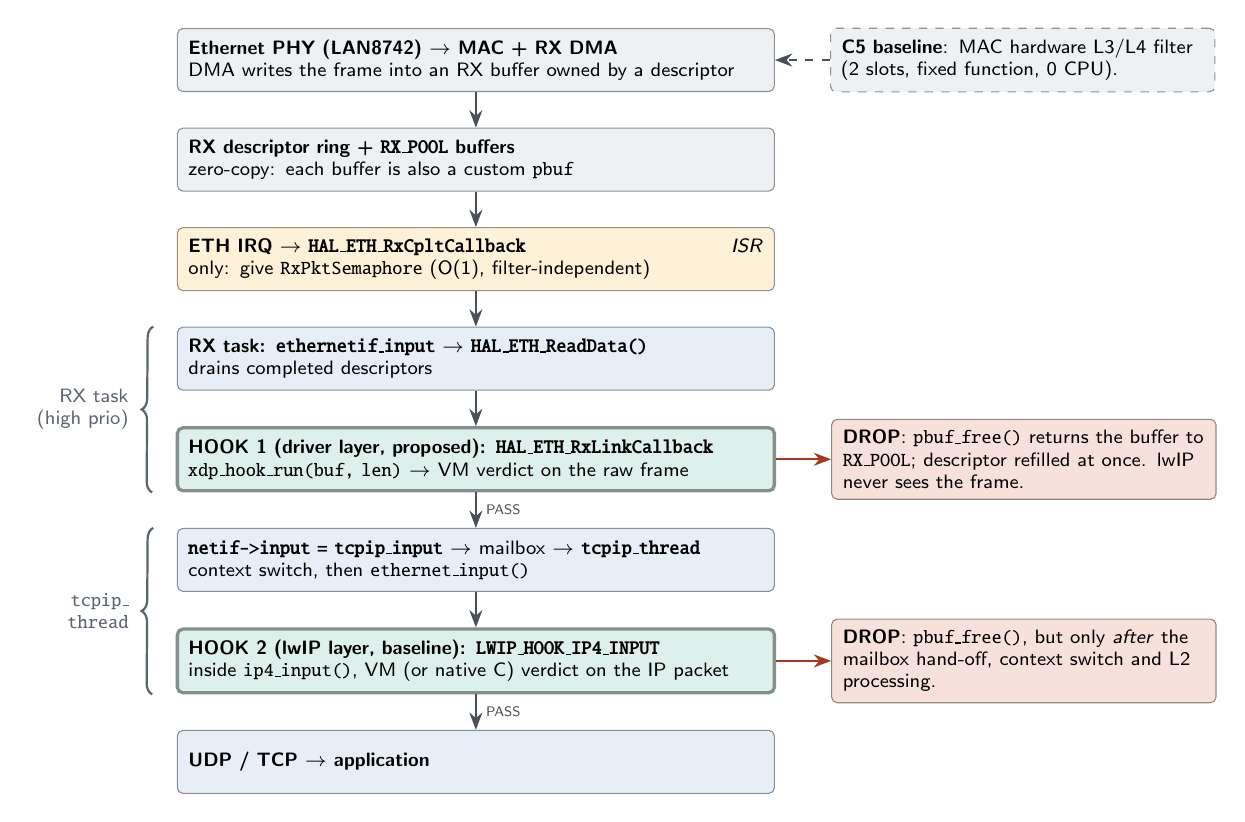
\begin{tikzpicture}[
  font=\sffamily\scriptsize,
  box/.style={draw=#1!60!black,fill=#1,rounded corners=2pt,align=left,text width=7.3cm,inner sep=4pt,minimum height=0.8cm},
  side/.style={draw=#1!60!black,fill=#1,rounded corners=2pt,align=left,text width=4.6cm,inner sep=4pt},
  arr/.style={-{Stealth[length=2.2mm]},thick,color=ink!80},
  node distance=4.5mm]
\node[box=hwfill]  (mac)  {\textbf{Ethernet PHY (LAN8742) $\rightarrow$ MAC + RX DMA}\\ DMA writes the frame into an RX buffer owned by a descriptor};
\node[box=hwfill,below=of mac] (ring) {\textbf{RX descriptor ring + \texttt{RX\_POOL} buffers}\\ zero-copy: each buffer is also a custom \texttt{pbuf}};
\node[box=isrfill,below=of ring] (isr) {\textbf{ETH IRQ $\rightarrow$ \texttt{HAL\_ETH\_RxCpltCallback}} \hfill \emph{ISR}\\ only: give \texttt{RxPktSemaphore} (O(1), filter-independent)};
\node[box=taskfill,below=of isr] (rxt) {\textbf{RX task: \texttt{ethernetif\_input} $\rightarrow$ \texttt{HAL\_ETH\_ReadData()}}\\ drains completed descriptors};
\node[box=hookfill,below=of rxt,very thick] (h1) {\textbf{HOOK 1 (driver layer, proposed): \texttt{HAL\_ETH\_RxLinkCallback}}\\ \texttt{xdp\_hook\_run(buf, len)} $\rightarrow$ VM verdict on the raw frame};
\node[box=taskfill,below=of h1] (tcp) {\textbf{\texttt{netif->input = tcpip\_input}} $\rightarrow$ mailbox $\rightarrow$ \textbf{\texttt{tcpip\_thread}}\\ context switch, then \texttt{ethernet\_input()}};
\node[box=hookfill,below=of tcp,very thick] (h2) {\textbf{HOOK 2 (lwIP layer, baseline): \texttt{LWIP\_HOOK\_IP4\_INPUT}}\\ inside \texttt{ip4\_input()}, VM (or native C) verdict on the IP packet};
\node[box=taskfill,below=of h2] (app) {\textbf{UDP / TCP $\rightarrow$ application}};

\node[side=dropfill,right=7mm of h1] (d1) {\textbf{DROP}: \texttt{pbuf\_free()} returns the buffer to \texttt{RX\_POOL}; descriptor refilled at once. lwIP never sees the frame.};
\node[side=dropfill,right=7mm of h2] (d2) {\textbf{DROP}: \texttt{pbuf\_free()}, but only \emph{after} the mailbox hand-off, context switch and L2 processing.};
\node[side=hwfill,right=7mm of mac,dashed] (hw) {\textbf{C5 baseline}: MAC hardware L3/L4 filter (2 slots, fixed function, 0 CPU).};

\draw[arr] (mac) -- (ring); \draw[arr] (ring) -- (isr); \draw[arr] (isr) -- (rxt);
\draw[arr] (rxt) -- (h1); \draw[arr] (h1) -- node[right,font=\sffamily\tiny]{PASS} (tcp);
\draw[arr] (tcp) -- (h2); \draw[arr] (h2) -- node[right,font=\sffamily\tiny]{PASS} (app);
\draw[arr,color=warn] (h1) -- (d1); \draw[arr,color=warn] (h2) -- (d2);
\draw[arr,dashed] (hw) -- (mac);

\draw[decorate,decoration={brace,amplitude=4pt,mirror},thick,color=muted]
  ([xshift=-3mm]rxt.north west) -- ([xshift=-3mm]h1.south west) node[midway,left=5pt,align=right,color=muted]{RX task\\(high prio)};
\draw[decorate,decoration={brace,amplitude=4pt,mirror},thick,color=muted]
  ([xshift=-3mm]tcp.north west) -- ([xshift=-3mm]h2.south west) node[midway,left=5pt,align=right,color=muted]{\texttt{tcpip\_}\\\texttt{thread}};
\end{tikzpicture}
\caption{Receive path on STM32H5 + FreeRTOS + lwIP, with the two VM hook points and the hardware filter baseline.}
\label{fig:rx}
\end{figure}

\subsection{The VM (Role 1)}
\textbf{Instruction format.} Fixed 64-bit instructions, \code{_Static_assert}-checked to 8 bytes:

\begin{center}
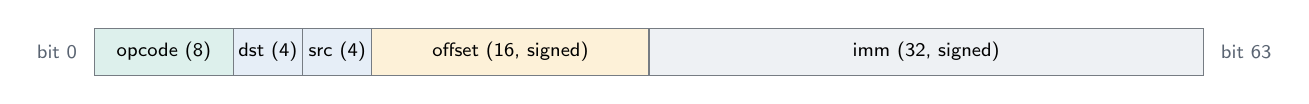
\begin{tikzpicture}[font=\sffamily\scriptsize]
\def\bw{0.22}
\foreach \x/\w/\t/\c in {0/8/{opcode (8)}/hookfill, 8/4/{dst (4)}/taskfill, 12/4/{src (4)}/taskfill, 16/16/{offset (16, signed)}/isrfill, 32/32/{imm (32, signed)}/hwfill}{
  \draw[fill=\c,draw=ink!60] (\x*\bw,0) rectangle ++(\w*\bw,0.6) node[pos=.5]{\t};
}
\node[anchor=east,color=muted] at (-0.1,0.3) {bit 0};
\node[anchor=west,color=muted] at (64*\bw+0.1,0.3) {bit 63};
\end{tikzpicture}
\end{center}

\begin{tabularx}{\textwidth}{@{}P{3.0cm}L@{}}
\toprule
Registers & 8 general-purpose 32-bit registers \code{r0..r7}, all zeroed at entry. \code{r0} is used as a 0 base for packet loads. There is no VM memory/stack in ISA v0. \\
Instruction classes & packet loads (\code{LDPKT_B/H/W}, big-endian), ALU with immediate or register (\code{ADD SUB AND OR XOR LSH RSH}), moves, conditional and unconditional branches (\code{JEQ JNE JGT JGE JLT JLE}, \code{JMP}), \code{RET} (verdict). Full table in Appendix~\ref{app:isa}. \\
Verdicts & \code{RET 1} = PASS, anything else = DROP. \\
\textbf{Verifier} (static) & non-empty, $\le 512$ instructions; known opcodes; registers $< 8$; every branch target in range and \textbf{strictly forward}; last instruction is \code{RET}. Forward-only branches make the control-flow graph a DAG, so every instruction runs at most once and \textbf{termination is guaranteed} in $\le n$ steps. \\
\textbf{Runtime checks} & every packet load checks \code{offset + size <= len} (frame length is only known at run time); a step budget is kept as defence in depth; NULL inputs are rejected. \textbf{Every fault resolves to DROP.} \\
Memory safety & The ISA has no pointers and no stores to memory. The only memory it can read is the frame, bounds-checked. A verified program cannot corrupt RTOS memory. \\
Interpreter & a single \code{switch} loop, which GCC compiles to one \code{TBH} jump table on Cortex-M33 (verified in the disassembly). Register file on the C stack, no heap, no globals. \\
\bottomrule
\end{tabularx}

\subsection{DDoS prototype bytecode (current, driver-layer variant)}
\begin{lstlisting}[style=bc]
; drop IPv4/UDP frames whose destination port == 1900 (SSDP amplification vector)
0:  ldpkt.h  r1, [r0+12]        ; EtherType
1:  jne      r1, 0x0800, +5     ; not IPv4      -> 7 (PASS)
2:  ldpkt.b  r2, [r0+23]        ; IPv4 protocol (assumes IHL = 5)
3:  jne      r2, 17, +3         ; not UDP       -> 7 (PASS)
4:  ldpkt.h  r3, [r0+36]        ; UDP destination port
5:  jne      r3, 1900, +1       ; other port    -> 7 (PASS)
6:  ret      0                  ; DROP          (7 instructions executed)
7:  ret      1                  ; PASS          (3 instructions for non-IPv4)
\end{lstlisting}
The lwIP-hook variant is the same logic with offsets shifted by 14 bytes (lwIP has already stripped the Ethernet header). Its limitations (UDP-only, IHL = 5, no VLAN, IP fragments) are listed in Section~\ref{sec:issues} and pinned by unit tests.

% =====================================================================
\needspace{22\baselineskip}
\section{Division of work}
% =====================================================================
The split below follows your two role descriptions (the screenshots) and the implementation guide. The ``going forward'' column is the proposed allocation for the rest of the MTP (details in \code{docs/ROADMAP.md}).

\begin{tabularx}{\textwidth}{@{}P{2.4cm}LL@{}}
\toprule
 & \textbf{Kiran (2025EET2800) --- Role 1} & \textbf{Nishant (2025EET2734) --- Role 2} \\
\midrule
\textbf{Title} & Virtual Machine as a Dynamic Execution Layer for Safe \& Deterministic Runtime & XDP-Inspired Packet Processing \& RTOS Network Integration \\
\textbf{Resume scope (as written)} & eBPF-like bytecode VM with custom ISA for packet processing, working with custom network hooks; lightweight verifier enforcing packet/memory bounds and bounded execution; interpreter optimised for CPU cycles, RAM and predictable latency; DDoS filter demo. & Ingress hook integrating the bytecode VM at the Ethernet RX/DMA driver layer, before lwIP; programmable PASS/DROP filtering with the lwIP IPv4 input hook for comparison; evaluation of latency, throughput, CPU, memory and RTOS overhead against native C; DDoS filtering prototype. \\
\textbf{Owns (code)} & \code{VM_Engine/}, \code{tests/host/}, \code{tools/asm/}, bytecode programs & \code{Network_Hooks/}, \code{Core/}, \code{LWIP/} integration, \code{bench/} \\
\textbf{Going forward} & ISA v1 spec; verify-on-install API; static min-length analysis (RQ3); Python assembler/disassembler; DDoS bytecode v1 (IHL, TCP+UDP, ports, fragments, VLAN); computed-goto vs switch benchmark; stateful rate-limit extension; verifier fuzzing. & Hardware bring-up; fix driver hook (D2--D7); lwIP hook via \code{LWIP_HOOK_FILENAME}; native-C baselines; \code{EXP_CONFIG} C0--C6; DWT/GPIO/run-time-stats instrumentation; traffic bench and flood sweeps; runtime program-update channel; ISR-placement experiment. \\
\textbf{Joint} & \multicolumn{2}{>{\raggedright\arraybackslash}p{13.4cm}}{DDoS demo end to end; evaluation design and analysis; MTP-1 report and final thesis (each writes their own chapters); optional workshop paper.} \\
\bottomrule
\end{tabularx}

\begin{keybox}{Interfaces between the two roles (agree on these early)}
\code{vm_verify(prog)} $\rightarrow$ result; \code{vm_interpreter_run(prog, frame, len, stats)} $\rightarrow$ verdict; \code{xdp_hook_run(frame, len)} $\rightarrow$ verdict (Nishant's wrapper); program install with verify-first and an atomic pointer swap; and the bytecode offset convention (the driver hook sees the Ethernet header, the lwIP hook sees the IP header). Changing any of these needs both of you to agree.
\end{keybox}

% =====================================================================
\section{What you shared, and the project history}
% =====================================================================
\subsection{Documents you shared with me}
\begin{tabularx}{\textwidth}{@{}P{4.6cm}L@{}}
\toprule
\textbf{Implementation guide} (PDF, 1 page) & Project overview; Role 1 (custom 64-bit ISA, verifier, optimised \code{switch} interpreter) and Role 2 (DMA ingress hook with zero-copy and instant descriptor free on DROP; lwIP \code{ip4_input()} hook as baseline; metrics); target directory structure (\code{Core/}, \code{VM_Engine/}, \code{Network_Hooks/}, \code{DDoS_Prototype/}). \\
\textbf{Two role-description screenshots} & Resume-style descriptions of Role 1 (Kiran) and Role 2 (Nishant), summarised in Section 5. \\
\textbf{Mid-term deck} (\code{Final_MTP_1.pptx}) & 11 slides, dated 24 Sep 2026: motivation, literature table, VM, verifier, DMA hook, dual-hook table, DDoS \& benchmarking, phase plan, conclusion, references. \\
\bottomrule
\end{tabularx}
All three are included in the bundle under \code{docs/reference/}.

\subsection{Papers studied so far: three}
The mid-term deck formally cites \textbf{three papers}: BPF (McCanne \& Jacobson, 1993) \cite{bpf93}, rBPF (Zandberg \& Baccelli, 2020) \cite{rbpf20}, and Femto-Containers (Zandberg \& Baccelli, 2021, arXiv) \cite{fc21}. All three citations in your deck are correct. It also discusses \textbf{Linux XDP} and \textbf{WebAssembly} as technologies without formal citations. Add \cite{xdp18} and \cite{wasm17} for those. Section~\ref{sec:lit} lists six more papers worth reading.

\subsection{Timeline}
\begin{tabularx}{\textwidth}{@{}P{2.7cm}L@{}}
\toprule
Before Sep 2026 & Topic and supervisor fixed; role split; literature (3 papers); implementation guide written. \\
Sep 2026 & v0 code drafted with Claude: \code{VM_Engine/}, \code{Network_Hooks/}, \code{DDoS_Prototype/}, integration notes. A Beamer version of the mid-term slides was started in that session but not finished. Your PowerPoint deck is the record of what was presented. (That draft also had a wrong author list for Femto-Containers; your deck's citation is the correct one.) \\
24 Sep 2026 & \textbf{Mid-term evaluation.} The deck's phase table records: Phase 1 \emph{completed} (architecture, literature review, baseline STM32H5 + FreeRTOS/lwIP setup); Phase 2 \emph{ongoing} (ISA, verifier, interpreter, Kiran); Phase 3 \emph{ongoing} (DMA hook and lwIP hook, Nishant); Phase 4 \emph{planned} (Python assembler, DDoS integration); Phase 5 \emph{planned} (benchmarking, thesis). \\
28 Oct 2026 & Audit and handoff (this dossier): v0.1 fix, 33 host unit tests, Cortex-M33 footprint numbers, compile checks of the hooks against the real HAL/lwIP/FreeRTOS headers, defect list, roadmap, \code{CLAUDE.md}. \\
\bottomrule
\end{tabularx}

\begin{warnbox}{What I can't know from here}
Whether the hardware baseline (Phase 1) actually runs on your board, which lwIP port and HAL version it uses, and whether any of the v0 code has been flashed since September. The first Claude Code session (Prompt A) starts by finding this out.
\end{warnbox}

% =====================================================================
\section{What has been built and verified}\label{sec:built}
% =====================================================================
\begin{tabularx}{\textwidth}{@{}P{4.4cm}P{2.1cm}L@{}}
\toprule
\textbf{Artefact} & \textbf{State} & \textbf{Evidence} \\
\midrule
\code{vm_isa.h} (ISA) & \done{} (v0.1) & Compiles host + CM33; \code{sizeof(vm_insn_t)==8} asserted. v0 lacked \code{<stddef.h>} and did not compile; fixed. \\
\code{vm_verifier.c} & \done{} & 9 accept/reject tests: backward jump, self-loop, out-of-range jump, bad opcode, bad register, missing RET, empty, NULL, over-length. \\
\code{vm_interpreter.c} & \done{} & Semantics tests (loads, ALU, reg-reg branches, negative offsets caught at run time, non-0/1 RET $\rightarrow$ DROP); runs clean under ASan + UBSan. \\
DDoS bytecode (2 variants) & \done{} (v0 rules) & DROP UDP$\rightarrow$1900; PASS UDP$\rightarrow$53, TCP$\rightarrow$1900, ARP, IPv6; runt/truncated frames $\rightarrow$ DROP (fail-safe). Limitations pinned by tests. \\
\code{lwip_ip4_hook.c} & compiles & Compiled against lwIP 2.2.x; lwIP \code{ip4.c} compiles with the hook via \code{LWIP_HOOK_FILENAME}. Not run on hardware. \\
\code{xdp_dma_hook.c} & \open{} & \textbf{Fails to compile} against the H5 HAL (D2) and has runtime blockers (D3--D6). \\
Host test suite & \done{} & \code{tests/host}: \textbf{33/33 pass}, also with \code{-fsanitize=address,undefined}. \\
Python assembler & not started & Planned (deck Phase 4). \\
Hardware integration / results & unknown & Not observed by me. \\
\bottomrule
\end{tabularx}

\subsection{Measured footprint on Cortex-M33 (arm-none-eabi-gcc 13.2.1, hard-float, \texttt{-Werror} clean)}
\begin{tabularx}{\textwidth}{@{}LP{2.2cm}P{2.2cm}P{2.6cm}P{2.2cm}@{}}
\toprule
\textbf{Object} & \textbf{.text -O2} & \textbf{.text -Os} & \textbf{Stack (-O2 / -Os)} & \textbf{.data/.bss} \\
\midrule
\code{vm_interpreter.o} & 1084 B & 932 B & 80 B / 72 B & 0 / 0 \\
\code{vm_verifier.o} & 463 B & 454 B & 16 B / 20 B & 0 / 0 \\
DDoS bytecode (both variants) & \multicolumn{2}{l}{$\approx$144 B (.rodata incl.\ accessors)} & --- & 0 / 0 \\
\bottomrule
\end{tabularx}
\textbf{Per-packet work:} the DROP path executes 7 VM instructions; non-IPv4 traffic exits after 3. \textbf{Claim supported:} ``the VM runs in under 1\,KB of RAM'' holds (an 80-byte stack frame, no static RAM). These are \emph{object-file} numbers. Re-measure in the final linked image and report cycles from DWT on the board.

% =====================================================================
\section{Known issues and deck-vs-code gaps}\label{sec:issues}
% =====================================================================
Full table with fixes: \code{docs/KNOWN_ISSUES.md}. The blockers in brief:

\begin{tabularx}{\textwidth}{@{}P{0.75cm}P{1.35cm}L@{}}
\toprule
\textbf{ID} & \textbf{Severity} & \textbf{Problem $\rightarrow$ fix} \\
\midrule
D1 & \textcolor{ok}{fixed} & Missing \code{<stddef.h>}: VM engine didn't compile $\rightarrow$ added. \\
D2 & Blocker & \code{HAL_ETH_RxAllocateCallback} must return \code{void} on H5 (failure = \code{*buff = NULL}). v0 returns a status $\rightarrow$ \emph{conflicting types} (confirmed). \\
D3 & Blocker & \code{pbuf_alloced_custom(..., NULL, ...)} writes through a NULL \code{pbuf_custom*} $\rightarrow$ HardFault on the first PASS frame. Use ST's \code{RxBuff_t}/\code{RX_POOL} design. \\
D4 & Blocker & No \code{custom_free_function}, and the pool is only 4 deep $\rightarrow$ RX stalls after $\sim$4 PASS frames. Free callback returns to pool; pool $>$ descriptor count. \\
D5 & Major & On DROP, \code{HAL_ETH_ReadData()} returns \code{HAL_OK} with \code{NULL}; ST's loop \code{while (p != NULL)} stops draining $\rightarrow$ stranded frames and latency spikes. Loop on the return status instead. \\
D6 & Major & v0 duplicates RX callbacks that ST's \code{ethernetif.c} already defines, and references a non-existent semaphore. Keep ST's callbacks; call \code{xdp_hook_run()} from inside \code{HAL_ETH_RxLinkCallback}; on DROP, \code{pbuf_free()} the custom pbuf. \\
D7 & Major & Including lwIP headers from \code{lwipopts.h} causes circular includes (confirmed). Use \code{LWIP_HOOK_FILENAME} (confirmed to compile). \\
\bottomrule
\end{tabularx}

\subsection{Mid-term deck vs implementation: fix before the next evaluation}
\begin{tabularx}{\textwidth}{@{}P{0.7cm}P{5.4cm}L@{}}
\toprule
\textbf{ID} & \textbf{Deck says} & \textbf{Reality / action} \\
\midrule
G1 & DMA hook runs \emph{in} the \code{RxCpltCallback} ISR & VM runs in the RX task via \code{RxLinkCallback}; ISR only signals. Correct the slides; optionally measure a VM-in-ISR variant (C6). \\
G2 & VM uses a ``fixed 512-byte stack'' & No VM stack exists (8 registers; 72--80\,B C frame). 512\,B is eBPF/rBPF's. Add a verified scratch stack or reword. \\
G3 & Verifier checks loads against packet length & That check is at run time. Say ``static + runtime'', or implement static min-length analysis (RQ3). \\
G4 & Drops ``TCP, UDP'' packets & Bytecode is UDP-only; extend it or reword. \\
G5 & ``Cortex-M3'' & Cortex-\textbf{M33}. \\
G6 & DMA hook: ``memory allocation: none'' & ST's custom pbuf is allocated with each RX buffer. The real saving is the skipped mailbox/context switch/L2 processing and early recycling. Measure it. \\
G7 & Python assembler & Not started; scheduled in the roadmap. \\
G8 & ``computed jump table (switch-case)'' & Accurate as ``jump-table switch'' (one \code{TBH}). True computed-goto dispatch would be a new optimisation to benchmark. \\
\bottomrule
\end{tabularx}

% =====================================================================
\needspace{12\baselineskip}
\section{Literature: studied, recommended, positioning}\label{sec:lit}
% =====================================================================
\subsection{The three papers you have studied}
\textbf{BPF --- McCanne \& Jacobson, USENIX Winter 1993} \cite{bpf93}. Introduced the in-kernel packet filter as a small \emph{register-based} virtual machine with a control-flow-graph filter model, replacing the older stack-based CSPF design. Filters run on the packet where it lies, before any copy to user space. \emph{Takeaway for you:} the ancestor of your design, and the origin of the ``filter early, filter in place'' argument.

\textbf{rBPF --- Zandberg \& Baccelli, PEMWN 2020} \cite{rbpf20}. A register-based eBPF-derived VM for low-power IoT microcontrollers (RIOT OS), compared against a WebAssembly interpreter. Reports that both VMs add execution-time overhead that is tolerable for low-throughput devices, while rBPF adds under 10\% memory in their networked case against roughly doubling it for WebAssembly. \emph{Takeaway:} evidence that a register VM is the right size class for an MCU.

\textbf{Femto-Containers --- Zandberg \& Baccelli, arXiv 2021} \cite{fc21}. Hosts multiple isolated eBPF-based VMs in RIOT as ``containers'', attached to OS hooks (launchpads), deployable over the network, with a 512-byte eBPF stack per VM. Reported measurements on an nRF52840 (Cortex-M4) running a fletcher32 checksum (verify these figures against the paper's tables before quoting them):

\begin{center}
\begin{tabular}{@{}lrrrr@{}}
\toprule
\textbf{Runtime} & \textbf{ROM} & \textbf{RAM} & \textbf{Startup} & \textbf{Run time} \\
\midrule
WASM3 (WebAssembly) & 64\,KiB & 85\,KiB & 17{,}096\,$\mu$s & 980\,$\mu$s \\
MicroPython & 101\,KiB & 8.2\,KiB & 21{,}907\,$\mu$s & 16{,}325\,$\mu$s \\
RIOTjs & 121\,KiB & 18\,KiB & 5{,}589\,$\mu$s & 14{,}726\,$\mu$s \\
rBPF & 4.4\,KiB & 0.6\,KiB & 1\,$\mu$s & 2{,}133\,$\mu$s \\
Native C & --- & --- & --- & 27\,$\mu$s \\
\bottomrule
\end{tabular}
\end{center}
\emph{Takeaway:} interpretation is slow for compute-heavy code (rBPF $\approx$77$\times$ native here), so your argument must rest on \emph{short} header filters and on \emph{where} they run, not on beating native C. That is RQ2. The peer-reviewed version is \cite{fc22} (Middleware '22). Cite both.

\subsection{Recommended next reading (six papers, in priority order)}
\begin{enumerate}[leftmargin=1.6em]
  \item \textbf{XDP --- Høiland-Jørgensen et al., CoNEXT 2018} \cite{xdp18}. The design you are porting: hook placement before buffer allocation, verdict actions, and how they evaluated it. Model your evaluation chapter on theirs.
  \item \textbf{Receive livelock --- Mogul \& Ramakrishnan, ACM TOCS 1997} \cite{mogul97}. Why interrupt-driven stacks collapse under load. This is the theory behind RQ4 and your flood plots.
  \item \textbf{Femto-Containers --- Zandberg et al., Middleware 2022} \cite{fc22}. The peer-reviewed, extended version with fault-isolation guarantees.
  \item \textbf{Verified rBPF --- Yuan et al., CAV 2022} \cite{cav22}. A mechanised proof of an eBPF VM for microcontrollers. Read it before claiming anything ``guaranteed'' about your verifier.
  \item \textbf{PREVAIL --- Gershuni et al., PLDI 2019} \cite{prevail19}. Static analysis of eBPF programs (abstract interpretation). Background for RQ3.
  \item \textbf{WebAssembly --- Haas et al., PLDI 2017} \cite{wasm17}. The primary source for the Wasm design you compare against.
\end{enumerate}

\subsection{Positioning}
\begin{tabularx}{\textwidth}{@{}P{2.5cm}P{2.5cm}LP{2.4cm}@{}}
\toprule
\textbf{System} & \textbf{Platform} & \textbf{Where it runs / safety} & \textbf{RAM class} \\
\midrule
Linux XDP/eBPF \cite{xdp18} & Linux servers, NIC drivers & NIC driver, before skb allocation; in-kernel verifier & MB \\
WebAssembly (WASM3) \cite{wasm17,fc21} & MCU, app level & sandboxed interpreter; not a network hook & tens of KiB \\
rBPF \cite{rbpf20} & RIOT, Cortex-M & OS hooks, low-rate IoT; runtime checks & $\sim$0.6\,KiB \\
Femto-Containers \cite{fc21,fc22} & RIOT; Cortex-M, ESP32, RISC-V & event hooks, OTA deployment; verified isolation \cite{cav22} & $\sim$0.66\,KiB/VM \\
MAC L3/L4 filter & STM32H5 MAC & hardware, 2 fixed-function slots & 0 \\
\textbf{This work} & \textbf{STM32H5, FreeRTOS + lwIP} & \textbf{Ethernet RX driver path, before lwIP (+ lwIP hook); static verifier + runtime bounds; fail-safe DROP} & \textbf{80\,B stack, 0 static} \\
\bottomrule
\end{tabularx}

% =====================================================================
\section{Evaluation plan}
% =====================================================================
Full version in \code{docs/EVALUATION_PLAN.md}. The core design is a 2$\times$2 grid plus bounds:

\begin{tabularx}{\textwidth}{@{}P{0.8cm}P{2.6cm}P{4.4cm}L@{}}
\toprule
\textbf{ID} & \textbf{Filter} & \textbf{Location} & \textbf{Purpose} \\
\midrule
C0 & none & --- & baseline lwIP under flood \\
C1 & native C & lwIP \code{ip4_input} hook & late placement, no interpretation \\
C2 & VM & lwIP \code{ip4_input} hook & late placement, interpreted \\
C3 & native C & driver hook & early placement, no interpretation \\
C4 & VM & driver hook & \textbf{proposed system} \\
C5 & hardware L3/L4 & Ethernet MAC & fixed-function lower bound \\
C6 & VM & ISR (experimental) & is ISR placement worth it? \\
\bottomrule
\end{tabularx}

\textbf{How to read it:} C1 vs C3 isolates \emph{placement}; C3 vs C4 isolates \emph{interpretation}; C4 vs C5 prices \emph{programmability} against hardware.

\textbf{Measurements:} DWT \code{CYCCNT} around the verdict (min/mean/p99/max); GPIO pulses from ISR entry to verdict on a logic analyser; FreeRTOS run-time stats and an idle-hook CPU-load counter; hook counters plus \code{ETH->DMACMFCR} for overruns; iperf goodput and ping RTT for legitimate traffic during floods; \code{arm-none-eabi-size}, the map file, \code{-fstack-usage} and stack high-water marks for footprint.

\begin{keybox}{The number that frames the whole thesis}
At 100\,Mbit/s a minimum-size frame occupies 84 bytes on the wire (64 + preamble + inter-frame gap), so line rate is $\approx$148{,}800 frames/s. At 250\,MHz that leaves
\[
  \frac{250\times10^{6}\ \text{cycles/s}}{148{,}800\ \text{frames/s}} \approx 1{,}680\ \text{cycles per frame}.
\]
Any per-frame path longer than this cannot keep up at line rate. Show where C0--C6 sit relative to this budget.
\end{keybox}

\textbf{Figures to produce:} (1) cycles per verdict, C1--C4 (bar + error bars); (2) CPU load vs flood rate; (3) legitimate goodput and RTT vs flood rate (the ``survivability'' plot); (4) RX overruns vs flood rate; (5) ISR-to-verdict latency histogram; (6) footprint table. Run each point at least 3 times, record spread, and keep every raw CSV with its git commit hash.

% =====================================================================
\section{Roadmap to the final thesis}
% =====================================================================
Assumption: MTP Part 1 ends with an evaluation in early December 2026, and Part 2 runs January--May 2027. Adjust to your calendar. Each milestone's definition of done is in \code{docs/ROADMAP.md}.

\begin{tabularx}{\textwidth}{@{}P{2.3cm}LL@{}}
\toprule
\textbf{When} & \textbf{Kiran} & \textbf{Nishant} \\
\midrule
M1 \,wk of 28 Oct & ISA v1 spec (\code{docs/ISA.md}); extend host tests & FreeRTOS + lwIP on the board (ping, UDP echo); pin versions; shared git repo \\
M2 \,wk of 4 Nov & verify-on-install (D9), D11; start static min-length analysis & fix D2--D7; lwIP hook via \code{LWIP_HOOK_FILENAME}; native-C filters \\
M3 \,wk of 11 Nov & Python assembler/disassembler; DDoS bytecode v1 & DWT/GPIO/run-time stats/\code{DMACMFCR}; \code{EXP_CONFIG}; PC flood bench \\
M4 \,wk of 18 Nov & \multicolumn{2}{>{\raggedright\arraybackslash}p{13.4cm}}{First runs C0--C4 at 3--5 flood rates; first plots generated by script} \\
M5 \,wk of 25 Nov & \multicolumn{2}{>{\raggedright\arraybackslash}p{13.4cm}}{Fix deck gaps G1--G8; MTP-1 report; 2-minute demo video} \\
\midrule
Jan 2027 & computed-goto vs switch; optional scratch stack & runtime program update over UDP (verify, double-buffer, atomic swap) \\
Feb 2027 & stateful rate-limit map; verifier fuzzing & full matrix incl.\ C5, C6; line-rate tests \\
Mar 2027 & \multicolumn{2}{>{\raggedright\arraybackslash}p{13.4cm}}{Thesis chapters (each your own); results analysis; optional workshop paper} \\
Apr--May 2027 & \multicolumn{2}{>{\raggedright\arraybackslash}p{13.4cm}}{Final numbers, reproducibility package, full draft to supervisor, submission and defence} \\
\bottomrule
\end{tabularx}

% =====================================================================
\section{Resume and interview material}
% =====================================================================
\begin{warnbox}{Rule}
Put a bullet on your resume only when it is true, and replace every [placeholder] with a \emph{measured} number from \code{eval/}. Interviewers will ask how you measured it.
\end{warnbox}

\textbf{Nishant --- Role 2 (XDP-Inspired Packet Processing \& RTOS Network Integration)}
\begin{itemize}
  \item Built an XDP-inspired ingress hook in the STM32H5 Ethernet RX driver path (Cortex-M33, FreeRTOS, lwIP) that runs verified bytecode filters on zero-copy DMA buffers and recycles dropped buffers before lwIP, cutting CPU cycles per dropped packet by [X]\% versus an lwIP \code{ip4_input} hook.
  \item Designed a 7-configuration evaluation (native C vs VM; driver vs lwIP vs MAC hardware filter) using DWT cycle counters, GPIO latency probes and FreeRTOS run-time stats; under a [Y]\,kpps UDP flood the board kept [Z]\% of legitimate goodput.
  \item Implemented a programmable DDoS filtering prototype with runtime filter updates over the network, with no reflash. \emph{(After the Jan 2027 milestone.)}
\end{itemize}

\textbf{Kiran --- Role 1 (VM as a Dynamic Execution Layer)}
\begin{itemize}
  \item Designed a 64-bit eBPF-like ISA and a heap-free interpreter for Cortex-M33 ($\approx$1\,KB flash, 80\,B stack, 0\,B static RAM) used as a programmable packet-filtering layer in a FreeRTOS/lwIP datapath. \emph{(Footprint numbers already measured.)}
  \item Implemented a static verifier guaranteeing termination (forward-only CFG) and memory safety (bounds-checked packet access, fail-safe DROP); static min-length analysis removed [N]\% of runtime checks / [M] cycles per packet.
  \item Built a Python assembler/disassembler and a host test suite ([K] tests, ASan/UBSan) for the bytecode toolchain.
\end{itemize}

\textbf{Talking points that work in interviews:} why early drop beats late drop (the 1,680-cycle budget); why the VM runs in a task and not the ISR; how forward-only branches give termination for free; what the MAC hardware filter can't do; one bug you found and how (D5's stranded frames is a good story).

% =====================================================================
\section{Viva / evaluation Q\&A preparation}
% =====================================================================
\newcommand{\qa}[2]{\textbf{Q: #1}\par\vspace{-1pt}\emph{A:} #2\par\vspace{3pt}}

\qa{Why not just write the filter in C and reflash?}{Programmability without reflash or reboot, and a safety guarantee for logic you didn't compile into the firmware. The price is interpretation overhead, which we measure directly (C3 vs C4).}
\qa{The STM32H5 MAC already filters TCP/UDP ports in hardware. Why a VM?}{It has two fixed-function slots with exact-match fields and no logic or state. We use it as the lower-bound baseline (C5). The VM handles port lists, header logic (IHL, fragments, VLAN) and, with the planned map extension, per-source rate limiting, none of which the hardware can do.}
\qa{How do you guarantee termination?}{The verifier only allows strictly forward branches, so the control-flow graph is a DAG and every instruction executes at most once: at most 512 steps. A runtime step budget remains as defence in depth.}
\qa{How do you guarantee memory safety?}{The ISA has no pointers and no memory stores. Register indices are verified, and the only readable memory is the frame, with every load bounds-checked against the frame length. Any fault forces DROP.}
\qa{Why doesn't the VM run in the interrupt, like Linux XDP in the driver?}{On an MCU the ISR must stay short and bounded, and lwIP's pbuf operations are not ISR-safe. Deferring to a high-priority RX task keeps interrupt latency independent of filter size. It is still the driver layer and still before lwIP. Experiment C6 quantifies the alternative.}
\qa{Is it really zero-copy?}{Yes. The VM reads the DMA buffer in place (pointer + length). On PASS the same buffer becomes the pbuf payload through ST's zero-copy RX pool. On DROP it returns to the pool and the descriptor is refilled.}
\qa{How much slower is the VM than native C?}{The literature reports large factors for compute-heavy code (rBPF $\approx$77$\times$ on fletcher32 \cite{fc21}). Our filters are 3--7 instructions, so the absolute cost per packet is what matters. We report measured cycles per verdict for both.}
\qa{Why is dropping at the driver cheaper?}{It skips the mailbox post to \code{tcpip_thread} and its context switch, \code{ethernet_input()} demultiplexing, and IP processing, and it returns the buffer to the RX ring sooner, so fewer overruns. RQ1 measures exactly this.}
\qa{Why a custom ISA instead of standard eBPF, which LLVM can already compile to?}{A smaller ISA makes a simpler, auditable verifier and a $\sim$1\,KB interpreter with 32-bit registers that match Cortex-M. The trade-off is no compiler, hence our assembler. Accepting a subset of standard eBPF is good future work.}
\qa{How do you update a filter safely at runtime?}{(Planned.) The new program arrives over a control channel with a CRC, is verified \emph{before} activation, and is installed into a second buffer. An aligned 32-bit pointer store then swaps it atomically on Cortex-M. The old program runs until the swap.}
\qa{What about IPv4 options, VLAN tags and fragments?}{Known limitations of the v0 bytecode, pinned by unit tests. Bytecode v1 parses IHL, skips non-first fragments and optionally handles 802.1Q.}
\qa{Any cache-coherency issue reading DMA buffers?}{The VM reads a buffer only after the DMA releases its descriptor (OWN bit clear) and the HAL hands it over. If that SRAM region were data-cacheable it would need cache maintenance. \emph{Before the viva, check in RM0481 whether the H5's caches cover the SRAM holding the RX buffers, and state the exact answer.}}
\qa{What exactly is new compared with Femto-Containers?}{The placement (high-speed Ethernet DMA receive path of FreeRTOS + lwIP rather than generic OS hooks on low-rate radios), the controlled placement-vs-interpretation-vs-hardware comparison, and (planned) verifier-driven removal of runtime checks.}
\qa{Who did what?}{Section 5: Kiran owns the ISA, verifier, interpreter and toolchain; Nishant owns the driver/lwIP integration, the RTOS side and the measurement bench; the demo and evaluation are joint.}

% =====================================================================
\section{Continuing in Claude Code}\label{sec:claudecode}
% =====================================================================
\begin{enumerate}
  \item Unzip \code{MTP_XDP_STM32.zip}. The folder that \emph{directly} contains \code{CLAUDE.md}, \code{docs/}, \code{firmware/} and \code{tests/} is your \textbf{project folder} (the ``repo root''). After a Windows ``Extract All'', use the inner folder if it is doubled.
  \item Back up your STM32CubeIDE project (the folder with the \code{.ioc} file), then move it into the project folder as \code{stm32_project/} and open it in CubeIDE from there, so only one copy exists.
  \item Open the project folder in Claude Code. Claude Code reads \code{CLAUDE.md} from the top of that folder at the start of every session, so the project context, ownership rules, verified HAL facts and integrity rules carry over without re-explaining.
  \item Paste \textbf{Prompt A} from \code{docs/KICKOFF_PROMPT.md}, after filling in its three placeholder lines. It begins with read-only discovery of your actual CubeIDE project (lwIP source, HAL version, RX loop, tools on your machine) and proposes a plan before changing anything. No need to attach this PDF; it is already in \code{docs/}.
  \item In later sessions, Kiran uses \textbf{Prompt B} and Nishant uses \textbf{Prompt C}. Each session ends by updating \code{CLAUDE.md} (status), \code{docs/LOG.md} and \code{docs/KNOWN_ISSUES.md}.
  \item Hardware stays in your hands. If Claude Code can't reach the ST-LINK or the serial port, it will tell you what to run and what to paste back.
\end{enumerate}

\appendix
% =====================================================================
\section{Bundle inventory}
% =====================================================================
\begin{tabularx}{\textwidth}{@{}P{6.2cm}L@{}}
\toprule
\code{CLAUDE.md} & project memory for Claude Code (repo root) \\
\code{README.md} & bundle index and changelog \\
\code{docs/Project_Dossier.pdf}, \code{.tex} & this document (and its LaTeX source, for Overleaf) \\
\code{docs/KICKOFF_PROMPT.md} & Prompts A (setup), B (Kiran), C (Nishant) \\
\code{docs/KNOWN_ISSUES.md} & D1--D12, filter limitations, G1--G8 \\
\code{docs/ROADMAP.md} & milestones and definitions of done \\
\code{docs/EVALUATION_PLAN.md} & RQs, C0--C6, metrics, traffic, reporting rules \\
\code{docs/LOG.md} & session log (first entry: this audit) \\
\code{docs/INTEGRATION_NOTES_v0.md} & original notes, annotated where superseded \\
\code{docs/reference/} & implementation guide, role screenshots, mid-term deck \\
\code{firmware/VM_Engine/} & \code{vm_isa.h}, \code{vm_verifier.[ch]}, \code{vm_interpreter.[ch]} \\
\code{firmware/Network_Hooks/} & \code{xdp_dma_hook.[ch]} (v0, blockers), \code{lwip_ip4_hook.[ch]} \\
\code{firmware/DDoS_Prototype/} & \code{ddos_bytecode.h}, \code{ddos_prototype_init.c} \\
\code{tests/host/} & \code{test_vm.c} (33 tests), \code{Makefile} (\code{run}, \code{asan}) \\
\bottomrule
\end{tabularx}

% =====================================================================
\needspace{18\baselineskip}
\section{ISA v0 opcode table}\label{app:isa}
% =====================================================================
Opcode = (sub-operation $\ll$ 3) $|$ class. Branch target = $pc + 1 + \text{offset}$ (forward only).

\begin{tabularx}{\textwidth}{@{}P{2.2cm}P{4.6cm}L@{}}
\toprule
\textbf{Class} & \textbf{Mnemonics (hex opcode)} & \textbf{Semantics} \\
\midrule
LD (0) & \code{LDPKT_B} 0x00, \code{LDPKT_H} 0x08, \code{LDPKT_W} 0x10 & \code{dst = pkt[src + off]}: 1/2/4 bytes, big-endian, bounds-checked \\
ALU\_K (1) & \code{ADD} 0x01, \code{SUB} 0x09, \code{AND} 0x11, \code{OR} 0x19, \code{XOR} 0x21, \code{LSH} 0x29, \code{RSH} 0x31 & \code{dst = dst op imm} (shifts masked to 0--31) \\
ALU\_X (2) & same sub-ops: 0x02 \ldots 0x32 & \code{dst = dst op src} \\
JMP\_K (3) & \code{JMP} 0x03, \code{JEQ} 0x0B, \code{JNE} 0x13, \code{JGT} 0x1B, \code{JGE} 0x23, \code{JLT} 0x2B, \code{JLE} 0x33 & if \code{dst cmp imm}: \code{pc += 1 + off} (unsigned compare) \\
JMP\_X (4) & \code{JEQ} 0x0C \ldots \code{JLE} 0x34 & if \code{dst cmp src}: \code{pc += 1 + off} \\
RET (5) & \code{RET} 0x05 & verdict = \code{imm} (1 = PASS, else DROP) \\
MISC (6) & \code{MOV_K} 0x06, \code{MOV_X} 0x0E & \code{dst = imm} / \code{dst = src} \\
\bottomrule
\end{tabularx}

% =====================================================================
\begin{thebibliography}{99}\small
\bibitem{bpf93} S.~McCanne and V.~Jacobson, ``The BSD Packet Filter: A New Architecture for User-level Packet Capture,'' in \emph{Proc. USENIX Winter 1993 Conference}, San Diego, CA, Jan.\ 1993. \textbf{[studied]}
\bibitem{rbpf20} K.~Zandberg and E.~Baccelli, ``Minimal Virtual Machines on IoT Microcontrollers: The Case of Berkeley Packet Filters with rBPF,'' in \emph{Proc. 9th IFIP Int. Conf. on Performance Evaluation and Modeling in Wireless Networks (PEMWN)}, Berlin, Germany, 2020, pp.~1--6. arXiv:2011.12047. \textbf{[studied]}
\bibitem{fc21} K.~Zandberg and E.~Baccelli, ``Femto-Containers: DevOps on Microcontrollers with Lightweight Virtualization \& Isolation for IoT Software Modules,'' arXiv:2106.12553, 2021. \textbf{[studied]}
\bibitem{fc22} K.~Zandberg, E.~Baccelli, S.~Yuan, F.~Besson, and J.-P.~Talpin, ``Femto-Containers: Lightweight Virtualization and Fault Isolation for Small Software Functions on Low-Power IoT Microcontrollers,'' in \emph{Proc. 23rd ACM/IFIP Int. Middleware Conference (Middleware '22)}, Quebec, Canada, 2022, pp.~161--173. doi:10.1145/3528535.3565242.
\bibitem{xdp18} T.~Høiland-Jørgensen, J.~D.~Brouer, D.~Borkmann, J.~Fastabend, T.~Herbert, D.~Ahern, and D.~Miller, ``The eXpress Data Path: Fast Programmable Packet Processing in the Operating System Kernel,'' in \emph{Proc. 14th ACM CoNEXT}, Heraklion, Greece, 2018, pp.~54--66. doi:10.1145/3281411.3281443.
\bibitem{mogul97} J.~C.~Mogul and K.~K.~Ramakrishnan, ``Eliminating Receive Livelock in an Interrupt-Driven Kernel,'' \emph{ACM Transactions on Computer Systems}, vol.~15, no.~3, 1997. (Earlier version: USENIX ATC 1996.)
\bibitem{cav22} S.~Yuan, F.~Besson, J.-P.~Talpin, S.~Hym, K.~Zandberg, and E.~Baccelli, ``End-to-End Mechanized Proof of an eBPF Virtual Machine for Micro-controllers,'' in \emph{Proc. Computer Aided Verification (CAV)}, 2022.
\bibitem{prevail19} E.~Gershuni, N.~Amit, A.~Gurfinkel, N.~Narodytska, J.~A.~Navas, N.~Rinetzky, L.~Ryzhyk, and M.~Sagiv, ``Simple and Precise Static Analysis of Untrusted Linux Kernel Extensions,'' in \emph{Proc. 40th ACM SIGPLAN PLDI}, Phoenix, AZ, 2019, pp.~1069--1084.
\bibitem{wasm17} A.~Haas \emph{et al.}, ``Bringing the Web up to Speed with WebAssembly,'' in \emph{Proc. 38th ACM SIGPLAN PLDI}, 2017.
\bibitem{st} STMicroelectronics: RM0481 (STM32H563/H573 reference manual); UM3115 (Nucleo-144 for STM32H5 user manual); \texttt{stm32h5xx-hal-driver} and \texttt{stm32h5-classic-coremw-apps} (GitHub); ``How to use the LwIP Ethernet middleware on the STM32H5 series'' (ST Community knowledge base).
\end{thebibliography}

\end{document}
